%! TeX program = lualatex
\documentclass[../main.tex]{subfiles}
\begin{document} \section{Discrete random variable}

A random variable is discrete if all possible values of \(X(\text{outcome})\) form a discrete set. Discrete random variable are described by their PMF or CDF which we introduce below. 

\begin{definition}[probability mass function (PMF)]
  The \hlmain{probability mass function} for a discrete random variable \(X\) is a nonnegative function \(f_{X}(x)\) that satisfies
  \[
    \mathbb{P}(X = x) \hspace{4in}
  \]
\end{definition}
\blanklines{5}

\faStar{} A valid PMF \(f_{X}\) must satisfy \(\sum_{i=1}^{n} f_{X}(x_{i}) = \underline{\hspace{1cm}}\) where \(x_{1},\ldots,x_{n}\) are all possible values of \(X\).
\blanklines{5}

\begin{example}
  Describe the PMF \(f_{X}\) for the discrete random variable \(X\) in Example~\ref{ex:random-variable-intro}.

  \begin{center}
    \begin{minipage}{0.25\textwidth}
      \begin{tabular}{l|l}
        Person & Height \\\midrule
        Zeus & \(165\) \\
        Hera & \(155\) \\
        Perseus & \(180\) \\
        Theseus & \(160\) \\
        Athena & \(170\) \\
        Poseidon  & \(170\) \\
        Hades & \(160\) \\
        Helios & \(170\) \\
        Selene & \(180\) \\
        Achilles & \(180\)
      \end{tabular}
    \end{minipage}
    \begin{minipage}{0.7\textwidth}
      \begin{tikzpicture}[scale=1]
        \begin{axis}[
          axis lines = middle, % boxed, middle
          height = {2.5in},
          width = {5in},
          label style={at={(ticklabel* cs:1)}},
          ymin={0}, ymax={1},
          xmin={0}, xmax={8},
          xtick={0,...,8}, xticklabels={\empty},
          ytick={0,0.2,0.4,0.6,0.8,1}, yticklabels={\empty},
          ]
        \end{axis}
      \end{tikzpicture}
    \end{minipage}
  \end{center}
  \blanklines{10}
\end{example}
\clearpage

\begin{example}
  Suppose we have an fair coin. The PMF for a discrete random variable \(X\) associating sequences of coin tosses to the number \(k\) of tosses required until a tail appears is
  \[
    f_{X}(k) = (1/2)^{k} \text{ for integers } k \ge 1.
  \]
  Take for granted that \(f_{X}\) is a valid probability mass function. 

  \begin{enumerate}[wide]
    \item What is the meaning of \(f_{X}(2)\) in the context of this question?
      \blanklines{5}
    \item What is the probability that at most \(3\) tosses are required before a tail appears?
      \blanklines{10}
  \end{enumerate}
\end{example}

\begin{example}
  Suppose a discrete random variable \(X\) takes values \(0,1,2\). Which of the following is a valid PMF for \(X\)?

  \begin{enumerate}[label=(\alph*)]
    \item \(f_{X}(0) = 1, f_{X}(1) = 2, f_{X}(2) = 3\).
    \item \(f_{X}(0) = 1/2, f_{X}(1) = 1/4, f_{X}(2) = 1/4\).
    \item \(f_{X}(0) = -1/2, f_{X}(1) = 1/2, f_{X}(2) = 1\).
    \item None of the above.
  \end{enumerate}
  \blanklines{5}
\end{example}

\begin{example}
  Suppose a PMF \(f_{X}(x)\) is given by \(f_{X}(3) = 1/7\), \(f_{X}(5)\) is unknown, and \(f_{X}(10) = 2/5\).  Find the unknown probability.
  \blanklines{5}
\end{example}

\clearpage

Sometimes, it's convenient to describe a discrete random variable by asking for the probability of the event \(X \le (\text{some value})\). 

\begin{definition}[cumulative distribution function (CDF)] \label{def:discrete-cdf}
  A function \(F_{X}(x)\) is a \hlmain{cumulative distribution function} for a discrete random variable if 
  \[
    \mathbb{P}(X \le x) \hspace{4in} % \mathbb{P}(X \le x).
  \]
\end{definition}
\blanklines{3}

\faStar{} A valid CDF must be non-decreasing and has \(\min( F_{X} ) = 0\) and \(\max ( F_{X} ) = 1\).

% Example~\ref{ex:discrete-random-varialbe-cdf-to-pmf} demonstrates that CDF and PMF contain the same information but merely present them differently.

\begin{example} \label{ex:discrete-random-varialbe-cdf-to-pmf}
  The CDF \(F_{X}\) of a random variable \(X\) is given below.

  \begin{minipage}{0.4\textwidth}
    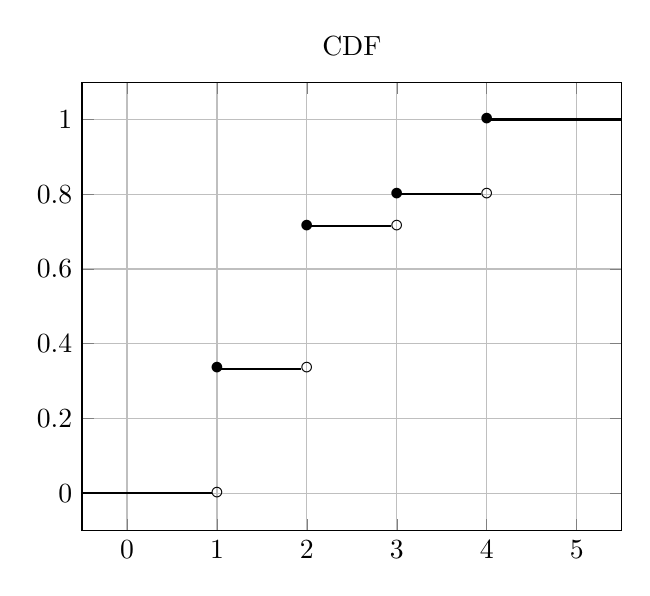
\begin{tikzpicture}
      \begin{axis}[grid=major, xmin=-0.5, xmax=5.5, title={CDF}]
        % \addplot[thick, black, mark=*] coordinates { (0,0) (0,0)};
        % \addplot[thick, black, mark=*] coordinates { (1,0) (1,1/2) };
        % \addplot[thick, black, mark=*] coordinates { (2,0) (2,3/4) };
        % \addplot[thick, black, mark=*] coordinates { (3,0) (3,7/8) };
        % \addplot[thick, black, mark=*] coordinates { (4,0) (4,1) };
        % \addplot[thick, black, mark=*] coordinates { (5,0) (5,1) };
        \addplot[thick, black] coordinates { (-1, 0)   (0.94, 0)  };
        \addplot[thick, black] coordinates { (1, 1/3)  (1.94, 1/3) };
        \addplot[thick, black] coordinates { (2, 5/7)  (2.94, 5/7) };
        \addplot[thick, black] coordinates { (3, 4/5)  (3.94, 4/5) };
        \addplot[thick, black] coordinates { (4, 1)    (5.94, 1)  };
        \node at (axis cs:1,0) {\(\circ\)};
        \node at (axis cs:2,1/3) {\(\circ\)};
        \node at (axis cs:3,5/7) {\(\circ\)};
        \node at (axis cs:4,4/5) {\(\circ\)};
        \node at (axis cs:1,1/3) {\(\bullet\)};
        \node at (axis cs:2,5/7) {\(\bullet\)};
        \node at (axis cs:3,4/5) {\(\bullet\)};
        \node at (axis cs:4,1) {\(\bullet\)};
      \end{axis}
    \end{tikzpicture}
  \end{minipage}
  \begin{minipage}{0.55\textwidth}
    \centering
    \begin{tikzpicture}
      \begin{axis}[
        axis lines = middle, % boxed, middle
        height = {2.5in},
        width = {3in},
        label style={at={(ticklabel* cs:1)}},
        ymin={0}, ymax={1},
        xmin={-0.5}, xmax={5.5},
        xtick={0,...,6}, xticklabels={0,1,2,3,4},
        ytick={0,0.2,0.4,0.6,0.8,1}, yticklabels={\empty},
        title={PMF}
        ]
      \end{axis}
    \end{tikzpicture}
  \end{minipage}
  \[
    F_{X}(0) = 0, \quad F_{X}(1) = 1/3,  \quad F_{X}(2) = 5/7,  \quad F_{X}(3) = 4/5,  \quad F_{X}(4) = 1.
  \]
  

  Find \(\mathbb{P}(X = 2)\) and \(\mathbb{P}(2 \le X \le 3)\).
  \blanklines{8}

  Describe the PMF for \(X\). Can you \emph{see} the PMF on the plot of CDF?
  \blanklines{8}
\end{example}
\clearpage

In general, we can easily convert between PMF and CDF for a discrete random variable \(X\). Suppose \(X\) takes values \(x_{1} < x_{2} < \cdots < x_{n}\).

\faStar{} If the PMF \(f_{X}\) is known, then its CDF \(F_{X}\) is
\blanklines{10}

\faStar{} If the CDF \(F_{X}\) is known, then its PMF \(f_{X}\) is
\blanklines{10}

We converted a CDF to a PMF in Example~\ref{ex:discrete-random-varialbe-cdf-to-pmf}. In the next example, we revert the process to convert from a PMF to a CDF.
\begin{example} \label{ex:discrete-random-varialbe-pmf-to-cdf}
  The PMF \(f_{X}\) of a random variable \(X\) is given below.
  \[
    f_{X}(1) = 1/3, \quad f_{X}(5) = 1/2, \quad f_{X}(7) = 1/6.
  \]

  Describe the CDF for \(X\) and sketch its PMF and CDF. Label the axes.

  \begin{minipage}{0.4\textwidth}
    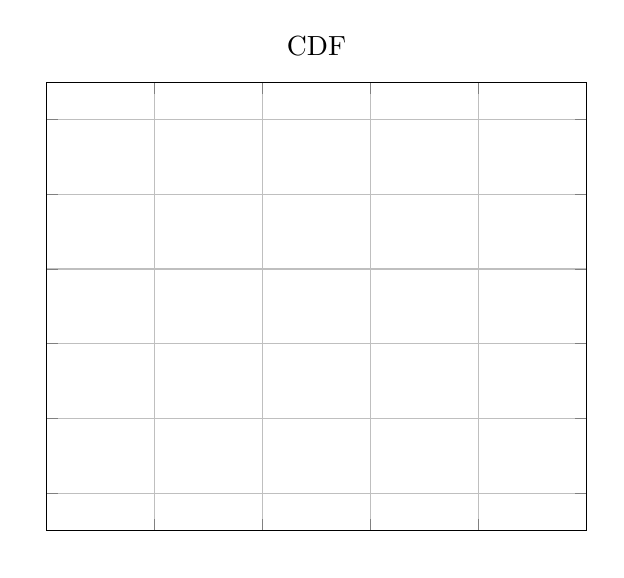
\begin{tikzpicture}
      \begin{axis}[grid=major, xmin=-0.5, xmax=5.5, xticklabels={\empty}, yticklabels={\empty}, title={CDF}]
        % % \addplot[thick, black, mark=*] coordinates { (0,0) (0,0)};
        % % \addplot[thick, black, mark=*] coordinates { (1,0) (1,1/2) };
        % % \addplot[thick, black, mark=*] coordinates { (2,0) (2,3/4) };
        % % \addplot[thick, black, mark=*] coordinates { (3,0) (3,7/8) };
        % % \addplot[thick, black, mark=*] coordinates { (4,0) (4,1) };
        % % \addplot[thick, black, mark=*] coordinates { (5,0) (5,1) };
        % \addplot[thick, black] coordinates { (-1, 0)   (0.94, 0)  };
        % \addplot[thick, black] coordinates { (1, 1/3)  (1.94, 1/3) };
        % \addplot[thick, black] coordinates { (2, 5/7)  (2.94, 5/7) };
        % \addplot[thick, black] coordinates { (3, 4/5)  (3.94, 4/5) };
        % \addplot[thick, black] coordinates { (4, 1)    (5.94, 1)  };
        % \node at (axis cs:1,0) {\(\circ\)};
        % \node at (axis cs:2,1/3) {\(\circ\)};
        % \node at (axis cs:3,5/7) {\(\circ\)};
        % \node at (axis cs:4,4/5) {\(\circ\)};
        % \node at (axis cs:1,1/3) {\(\bullet\)};
        % \node at (axis cs:2,5/7) {\(\bullet\)};
        % \node at (axis cs:3,4/5) {\(\bullet\)};
        % \node at (axis cs:4,1) {\(\bullet\)};
      \end{axis}
    \end{tikzpicture}
  \end{minipage}
  \begin{minipage}{0.55\textwidth}
    \centering
    \begin{tikzpicture}
      \begin{axis}[
        axis lines = middle, % boxed, middle
        height = {2.5in},
        width = {3in},
        label style={at={(ticklabel* cs:1)}},
        ymin={0}, ymax={1},
        xmin={-0.5}, xmax={5.5},
        xtick={0,...,6}, xticklabels={\empty},
        ytick={0,0.2,0.4,0.6,0.8,1}, yticklabels={\empty},
        title={PMF}
        ]
      \end{axis}
    \end{tikzpicture}
  \end{minipage}
  \blanklines{5}
\end{example}

\end{document}
